%---------change this for every latex homework
\def\yourid{rtg5xkh}
\def\collabs{}
\def\sources{Cormen, et al, Introduction to Algorithms. }
% -----------------------------------------------------
\def\duedate{Friday, April 8, 2022 at 11:30 pm }
\def\duelocation{via Gradescope}
\def\htype{Adv}
\def\hunit{B}
\def\hnumber{}
\def\course{{cs4102 - algorithms - spring 2022}}%------
%-------------------------------------
%-------------------------------------

\documentclass[10pt]{article}
\usepackage[colorlinks,urlcolor=blue]{hyperref}
\usepackage[osf]{mathpazo}
\usepackage{amsmath,amsfonts,amssymb, graphicx}
\usepackage{latexsym}
\usepackage[top=1in,bottom=1.4in,left=1.25in,right=1.25in,centering,letterpaper]{geometry}
\usepackage{color}
\definecolor{mdb}{rgb}{0.1,0.6,0.4} 
\definecolor{cit}{rgb}{0.05,0.2,0.45} 
\pagestyle{myheadings}
\markboth{\yourid}{\yourid}
\usepackage{clrscode}
\usepackage{tabularx}
\newcolumntype{Y}{>{\centering\arraybackslash}X}

\newenvironment{proof}{\par\noindent{\it Proof.}\hspace*{1em}}{$\Box$\bigskip}
\newcommand{\handout}{
   \renewcommand{\thepage}{Unit \hunit: \htype~Homework \hnumber~-~\arabic{page}}
   \noindent
   \begin{center}
      \vbox{
    \hbox to \columnwidth {\sc{\course} \hfill}
    \vspace{-2mm}
       \hbox to \columnwidth {\sc due \MakeLowercase{\duedate} \duelocation\hfill {\Huge\color{mdb}\hunit\hnumber{\Large\MakeLowercase{\htype}}(\yourid)}}
      }
   \end{center}
   \vspace*{1mm}
   \hrule
   \vspace*{1mm}
    {\footnotesize \textbf{Collaboration Policy:} You are encouraged to collaborate with up to 3 other students, but all work submitted must be your own {\em independently} written solution. List the computing ids of all of your collaborators in the \texttt{collabs} command at the top of the tex file. Do not share written notes, documents (including Google docs, Overleaf docs, discussion notes, PDFs), or code.  Do not seek published or online solutions for any assignments. If you use any published or online resources (which may not include solutions) when completing this assignment, be sure to cite by naming the book etc.\ or listing a website's URL. Do not submit a solution that you are unable to explain orally to a member of the course staff. Any solutions that share similar text/code will be considered in breach of this policy. Please refer to the syllabus for a complete description of the collaboration policy.
   \vspace*{1mm}
    \hrule
    \vspace*{2mm}
    \noindent
    \textbf{Collaborators}: \collabs\\
    \textbf{Sources}: \sources}
    \vspace*{2mm}
    \hrule
    \vskip 2em
}

\newcommand{\solution}[1]{\color{blue}\hfill\break\noindent\textbf{Solution:} #1\color{black}}
%\newcommand{\altsolution}[1]{\color{blue}\hfill\break\noindent\textbf{Solution (Alternative):} #1\color{black}}

%\newcommand{\solution}[1]{}
\newcommand{\altsolution}[1]{}

\newcommand{\bit}[1]{\{0,1\}^{ #1 }}
%\dontprintsemicolon
%\linesnumbered
\newtheorem{problem}{\sc\color{cit}problem}
\newtheorem{practice}{\sc\color{cit}practice}
\newtheorem{lemma}{Lemma}
\newtheorem{definition}{Definition}
\newtheorem{theorem}{Theorem}

\newcommand{\Z}{\mathbb{Z}} % This might be useful for Integers!

\begin{document}
\thispagestyle{empty}
\handout

%----Begin your modifications here


%--------------------------------------------------------------------------
\begin{problem}Proof about MSTs\end{problem}

Let $e=(u,v)$ be a minimum-weight edge in an undirected connected graph $G$. Prove that $e=(u,v)$ belongs to some minimum spanning tree of G. 

\solution{
    \begin{proof}
    
        Assume that e is not in any minimum spanning tree of G. \\
        Thus, there must exist a valid MST that does not contain e. Consider such an MST. If we were to add e to it, we would form a cycle, and there would be now be v total edges. To get rid of the cycle and form another MST, we will select the edge in the cycle with maximum weight and remove it. This edge that we are removing cannot be e, because e has the minimum weight of all the edges in the graph (and if there is a tie for the maximum, we will choose to remove an edge other than e). You will notice that, since we removed an edge and added one, the new MST has v-1 edges like it should. Additionally, since we created one cycle and removed that same cycle, the MST will not contain any cycles, thus it is valid. \\
        \null \quad There are 2 cases we must consider for the edge we removed and replaced with e: \\
        \null \quad If the edge from the original MST we removed has the same weight as e, we have constructed a new minimum spanning tree with the same total cost as the original MST we considered, thus this new MST containing e is valid, and we have reached a contradiction. \\
        \null \quad Otherwise, if the edge we removed had a weight that's greater than e, by removing it from the tree and adding e, we have constructed an MST with a total cost that is less than the original MST. Thus, the MST we were considering was actually not a valid MST. This is a contradiction. \\
        \null \quad Thus, since assuming e is not in any MST of G led to a contradiction, it must be true that e belongs to some minimum spanning tree of G.
        
        

    \end{proof}
}

\pagebreak

%--------------------------------------------------------------------------
\begin{problem}\end{problem}

An airline, Gamma Airlines, is analyzing their network of airport connections.  They have a graph $G=(A,E)$ that represents the set of airports $A$ and their flight connections $E$ between them. They define $hops(a_i, a_k)$ to be the smallest number of flight connections between two airports.  They define $maxHops(a_i)$ to be the number of hops to the airport that is farthest from $a_i$, i.e. $maxHops(a_i) = max( hops(a_i, a_j) )\, \forall a_j \in A$.

The airline wishes to define one or more of their airports to be ``Core 1 airports.'' Each Core 1 airport $a_i$ will have a value of $maxHops(a_i)$ that is no larger than any other airport.  You can think of the Core 1 airports as being ``in the middle'' of Gamma Airlines' airport network.  The worst flight from a Core 1 airport (where ``worst'' means having a large number of connections) is the same or better than any other airport's worst flight connection (i.e.\ its $maxHops()$ value).

They also define ``Core 2 airports'' to be the set of airports that have a $maxHops()$ value that is just 1 more than that of the Core 1 airports.  (Why do they care about all this?  Delays at Core 1 or Core 2 airports may have big effects on the overall network performance.)

\textbf{Your problem: } Describe an algorithm that finds the set of Core 1 airports and the set of Core 2 airports.  Give its time-complexity.   The input is $G=(A,E)$, an undirected and unweighted graph, where $e = (a_i, a_j) \in E$ means that there is a flight between $a_i$ and $a_j$. Base your algorithm design on algorithms we have studied in this unit of the course.

\solution{ \\
\null \quad To identify all of the Core 1 and Core 2 airports, We will need to find the value of $maxHops(a_i)$ For each airport $a_i$ and compare these values. To do this, we can use Breadth First Search on each airport in the graph. The depth of the resulting tree will represent the number of connecting flights from that airport to it's furthest airport. This is because in a BFS tree, each path from the start vertex, $s$, to any other vertex, $v_i$, in the tree represents the shortest path (in terms of number of edges) from $s$ to $v_i$. Thus, the depth of the BFS tree for any given airport, $a$, will capture the shortest path from $a$ to the airport furthest from $a$. This is exactly what $maxHops(a_i)$ specifies. We can find the depth of the tree after BFS completes simply by traversing through it. We will assign these depths as variables belonging to each airport for easy access. We will also keep track of the minimum BFS tree depth in this step, where if an airport has a depth that is less than the current minimum, we will set the minimum to be that new value.  \\
\null \quad Once BFS has been run on every airport in the network and we have established all of the $maxHops$ values, we will run through each airport in the graph once again to determine the Core 1 and Core 2 airports. For each airport a, if  $maxHops(a)$ is equal to the minimum, we'll add it to the set of Core 1 airports. Else if $maxHops(a)$ is equal to the minimum + 1, we'll add it to the set of Core 2 airports. \\ \\
Time complexity: \\
\null \quad The first step iterates through all airports, running BFS and traversing the resulting tree for each one. BFS's time complexity is $\Theta(V+E)$, and the tree traversal step is $O(V)$ so this step in total will be $\Theta(A*(A+E+A)$, where A is the number of airports and E is the number of flight connections. The next step that traverses the network again just runs through each airport and does one check so it will simply be $\Theta(A)$. \\ 
\null \quad Thus the overall time complexity for this algorithm is $\Theta(A^2 + AE)$.
}

\pagebreak

%--------------------------------------------------------------------------
\begin{problem}Vulnerable Network Nodes\end{problem}

Your security team has a model of nodes $v_i$ in your network where the relationship $d(v_i, v_j)$ defines if $v_j$ \emph{depends} on $v_i$. That is, if $d(v_i, v_j)$ is true,  the availability of second of these, $v_j$ relies on or depends on the availability of the first, $v_i$. We can represent this model of dependencies as a graph $G=(V,E)$ where $V$ is the set of network nodes and $e=(v_i, v_j) \in E$ means that $d(v_i, v_j)$ is true.  (For example, in the graph below, both H and J depend on F.)

Your team defines a \emph{vulnerable set} to be a subset $V'$ of the nodes in $V$ where all nodes in the subset depend on each other either directly or indirectly. (By ``indirectly'', we mean that $d(v_i, v_j)$ is not true, but $v_j$ depends on another node which eventually depends on $v_i$, perhaps through a ``chain'' of dependencies. For example, in the graph below, F depends on D indirectly.) 

\textbf{Your problem:}  Describe an algorithm (\textbf{and} give its time complexity) that finds the vulnerable set $VM$ in $G$ where 
\begin{enumerate}
\item the number of nodes in $VM$ is no smaller than the number of nodes in any other vulnerable set found in $G$, and
\item $\nexists \, v_i \in VM \textrm{ and } v_j \notin VM \textrm{ s.t. } d(v_i, v_j)$
\end{enumerate}
The second condition means that there are no nodes outside of VM that depend on any node in VM.

For example, in the graph below, there are a number of vulnerable sets, including $\{D, E, F\}, \{J, K\}$ and $\{G, H, I\}$.   The first of these does not meet the second condition. The other two do, but the last one is larger than the second one, so $VM=\{G, H, I\}$.

 
 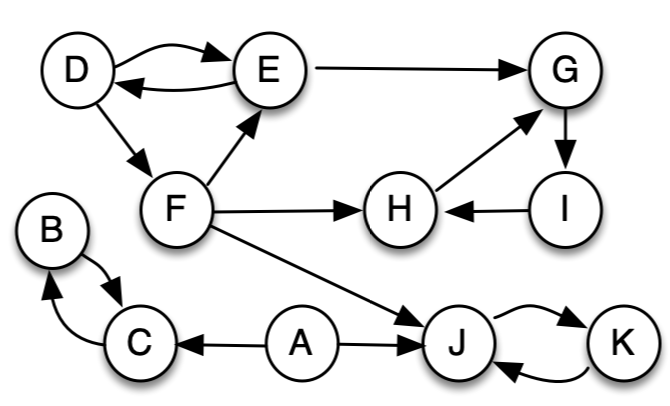
\includegraphics[width = 0.4\columnwidth]{vulnerable-sets.png}

\solution{ \\
\null \quad My algorithm will first find all strongly connected components of G. To do this, It will call DFS-sweep on G, recording all of the finishing times and assigning those finish times to each node for easy access. Next, it will compute $G^T$, the transpose graph of G. Then, it will again call DFS-sweep, but this time on $G^T$, and it will make the recursive calls to DFS-sweep in the reverse order of the times of the nodes. That is, in the for loop in DFS-sweep that calls DFS-visit on a certain node if it is unseen, I will ensure that the for loop begins with the node with the highest finishing times and goes down from there. This can be done by creating a list of nodes in sorted order of their finishing times in the first DFS-sweep call (on G), and simply traversing backwards through that list in this step. This doesn't increase the time complexity of DFS-sweep because it can simply add to the list once each time a finishing time is set. The forest of node trees that is produced by this DFS-sweep (on $G^T$) is the set of strongly connected components (SCCs) of the Network. While determining the SCCs, we will also make sure to keep a counter in the for loop of DFS-sweep, and pass this counter along to DFS-visit, which will assign that counter value to each node that it visits. This way, each node will have a identifier that can tell us which SCC it is in. This will be important later. The counter will not add any time complexity to DFS-sweep either. \\ 
Since a vulnerable set is defined to be a subset of nodes where each one either directly or indirectly depends on all other nodes in that set, by identifying the SCCs of the graph we have also identified all of the vulnerable sets (the SCCs and the vulnerable sets will be the same because they both are essentially defined by each node being reachable by every other node in a certain subset of a graph). \\
Next, we will check the conditions for each vulnerable set. To do this, we will iterate through each node in the Original Graph G once again. For each node n, we will first check d(n, a) on each adjacent node a in the Original graph, G. If d(n, a) is True AND the SCC identifier for d and a (we established this above) doesn't match, then we can eliminate any nodes in the same vulnerable set as this node. We will keep track of this and in the future if we see any nodes which have the same SCC identifier as one that's been eliminated, we can simply move on to the next one because that vulnerable set doesn't satisfy the second condition. During our iteration, we will also keep a counter to count the number of nodes that we encounter in each vulnerable set using their identifiers. Once this process is complete, we will return the vulnerable set that (1) has not been eliminated due to an outward dependency and (2) has the maximum number of nodes of the remaining vulnerable sets. \\ \\
Time complexity: \\
\null \quad We can find the time complexity by breaking the algorithm's steps into pieces. First, it runs DFS-Sweep on the graph, which is $\Theta(V+E)$. Next, we compute the transpose graph of G, which is also $\Theta(V+E)$, because it will visit each vertex and each edge in the graph once. Then, we perform DFS-sweep again to find the vulnerable sets. Finally, we iterate through each vertex in the graph once again, checking each of its outbound edges, which will visit each vertex and each edge. This is also $\Theta(E + V)$. \\ 
\null \quad Thus the total time complexity for this algorithm is $4(E+V) \in \Theta(E + V)$.
} \\

\begin{problem} Gradescope Submission \end{problem}
Submit a version of this \verb|.tex| file to Gradescope with your solutions added, along with the compiled PDF.  You should only submit your \verb|.pdf| and \verb|.tex| files.


\end{document}

